\documentclass{article}
\usepackage[margin=0.5in]{geometry}
\usepackage[utf8]{inputenc}
%\usepackage{textcomp}

\usepackage{pgfplots}
\pgfplotsset{width=10cm,compat=1.9}

%\usepgfplotslibrary{external}
%\tikzexternalize

\begin{document}
\begin{enumerate}

\item The histogram below shows the heart rate $x$ in beats per minute for 65 athletes after a fitness exercise. \hfill [2 points]

	\begin{center}
		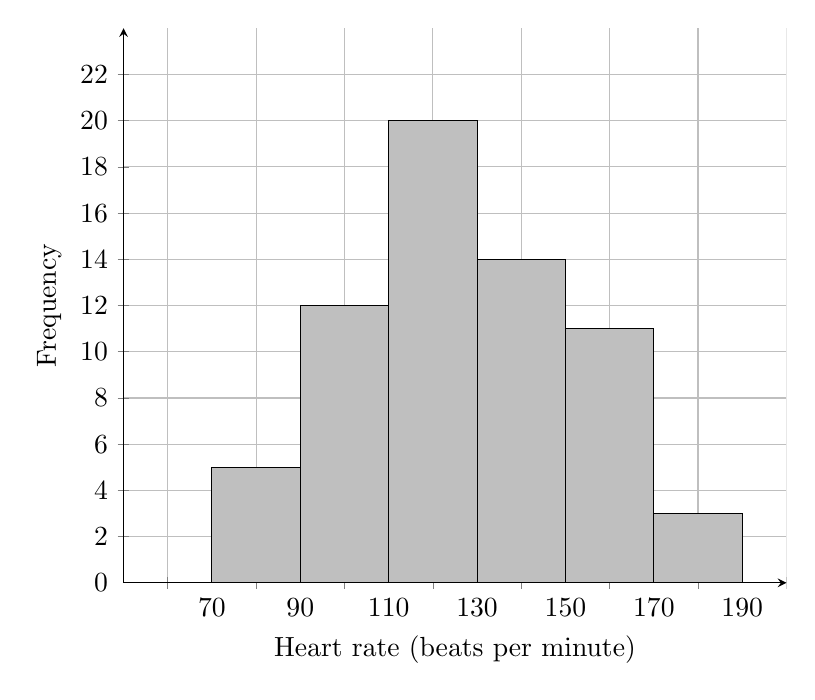
\begin{tikzpicture}
		\begin{axis}[
			xlabel=Heart rate (beats per minute),
			ylabel=Frequency,
			ybar interval=1,
			xmin=60, xmax=210,
			ymin=0, ymax=24,
			xtick={70,90,110,130,150,170,190,210},
			ytick={0,2,4,6,8,10,12,14,16,18,20,22},
			axis lines = left,
			ymajorgrids=true,
		]
		\addplot+ [color=black, fill=lightgray]
			coordinates {(80,5) (100,12)
				(120,20) (140,14) 
				(160,11) (180,3)
				(200,3)}; %Last pair does not show
		\end{axis}
		\end{tikzpicture}
	\end{center}

	The following is the frequency table for the distribution of $x$.
	\begin{center}
		\begin{tabular}{|l|c|c|c|c|c|c|}
			\hline
			Heart rate ($x$) & $70 \leq x < 90$ & $90 \leq x < 110$ & $110 \leq x < 130$ & $130 \leq x < 150$ & $150 \leq x < 170$ & $170 \leq x < 190$\\ 
			\hline 
			Frequency & 5 & 12 & 20 & 14 & 11 & 3 \\ 
			\hline 
			\end{tabular}
		\end{center}

\item Bar chart:

	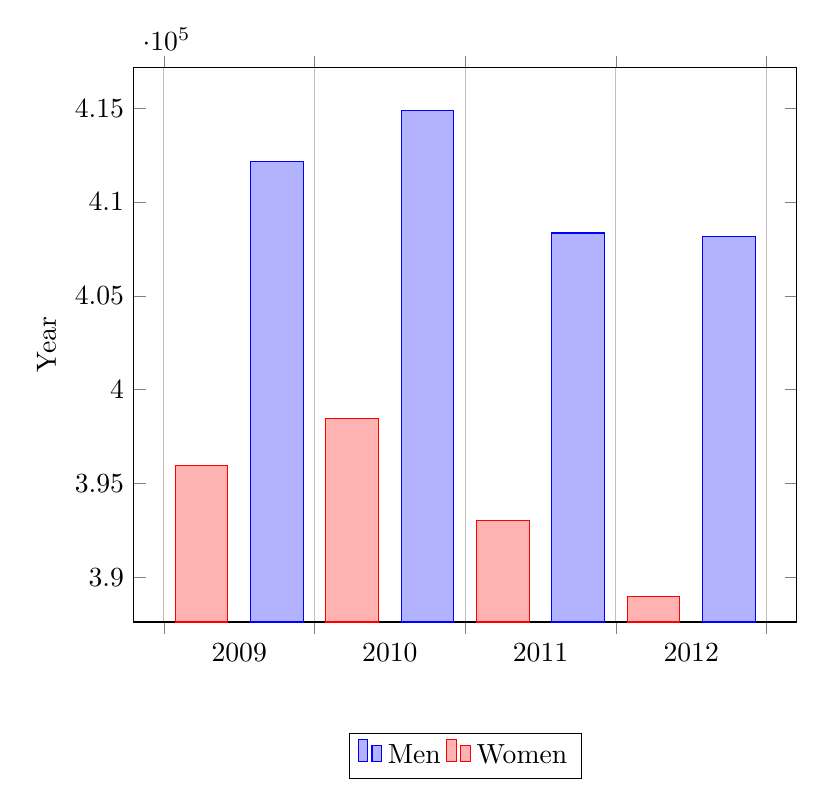
\begin{tikzpicture}
	\begin{axis}[
		x tick label style={
			/pgf/number format/1000 sep=},
		ylabel=Year,
		enlargelimits=0.05,
		legend style={at={(0.5,-0.2)},
		anchor=north,legend columns=-1},
		ybar interval=.7,
	]
	\addplot 
		coordinates {(2012,408184) (2011,408348)
			(2010,414870) (2009,412156) (2008,415838)};
	\addplot 
		coordinates {(2012,388950) (2011,393007) 
			(2010,398449) (2009,395972) (2008,398866)};
	\legend{Men,Women}
	\end{axis}
	\end{tikzpicture}

\end{enumerate}
\end{document}
